%% Template for MLP Coursework 1 / 16 October 2017 

%% Based on  LaTeX template for ICML 2017 - example_paper.tex at 
%%  https://2017.icml.cc/Conferences/2017/StyleAuthorInstructions

\documentclass{article}

\usepackage[T1]{fontenc}
\usepackage{amssymb,amsmath}
\usepackage{txfonts}
\usepackage{microtype}

% For figures
\usepackage{graphicx}
\usepackage{subfigure} 

% For citations
\usepackage{natbib}

% For algorithms
\usepackage{algorithm}
\usepackage{algorithmic}

% the hyperref package is used to produce hyperlinks in the
% resulting PDF.  If this breaks your system, please commend out the
% following usepackage line and replace \usepackage{mlp2017} with
% \usepackage[nohyperref]{mlp2017} below.
\usepackage{hyperref}
\usepackage{url}
\urlstyle{same}

% Packages hyperref and algorithmic misbehave sometimes.  We can fix
% this with the following command.
\newcommand{\theHalgorithm}{\arabic{algorithm}}


% Set up MLP coursework style (based on ICML style)
\usepackage{mlp2017}
\mlptitlerunning{MLP Coursework 1 (\studentNumber)}
\bibliographystyle{icml2017}


\DeclareMathOperator{\softmax}{softmax}
\DeclareMathOperator{\sigmoid}{sigmoid}
\DeclareMathOperator{\sgn}{sgn}
\DeclareMathOperator{\relu}{relu}
\DeclareMathOperator{\lrelu}{lrelu}
\DeclareMathOperator{\elu}{elu}
\DeclareMathOperator{\selu}{selu}
\DeclareMathOperator{\maxout}{maxout}

%% You probably do not need to change anything above this comment

%% REPLACE this with your student number
\def\studentNumber{s1794066}

\begin{document} 

\twocolumn[
\mlptitle{MLP Coursework 1: Activation Functions}

\centerline{\studentNumber}

\vskip 7mm
]

\begin{abstract} 
This report compares the effects of using four different activation functions in the hidden layers of a neural network. As a baseline, we used the same architecture, but with a sigmoidal activation function. We also investigate the effects of network depth, and weights initialisation strategies. Evaluated by validation set accuracy on the MNIST dataset, we find Leaky ReLU to perform the best of the activation functions. We also find that using 7 layers and a Glorot weights initialisation scheme gives us the highest validation set accuracy. 
\end{abstract} 

\section{Introduction}
\label{sec:intro}
Neural networks have been used extensively for classification problems in machine learning. They can be evaluated for an input $\mathbf{x} \in \mathrm{R}^{Dx1}$ for $l = {1, \dots, L+1}$
\begin{align*}
\mathbf{h}^{(1)} &= W^{(1)}\mathbf{x} + \mathbf{b}^{(1)}
\\
\mathbf{a}^{(1)} &= \mathbf{g}^{(1)} (\mathbf{h}^{(1)})
\\
\mathbf{h}^{(l)} &= W^{(l)}\mathbf{a}^{(l-1)} + \mathbf{b}^{(l)}
\\
\mathbf{a}^{(l)} &= \mathbf{g}^{(l)} (\mathbf{h}^{(l)})
\\ 
\mathbf{f(\mathbf{x})} &= \mathbf{a}^{(L+1)}
 \end{align*}
 where $L$ is the number of hidden layers in the network. If $K^{(l)}$ is the dimensionality of hidden layer $l$, then $W^{(l)} \in \mathrm{R}^{K^{(l)}xK^{(l-1)}}$ and $b \in \mathrm{R}^{K^{(l)}}$. In supervised learning, there is a training dataset with training examples $\mathbf{x}^{(m)}$ and target outputs $\mathbf{y}^{(m)}$.  An associated error function $E$ which depends on $\mathbf{x}^{(m)}$, $\mathbf{y}^{(m)}$ and the weights matrices $W^{(l)}$ is used to evaluate predictions of the network, and subsequently train the weights. 
 
The choice of function $\mathbf{g}^{(l)}$ is an important one. First of all, it must be non-linear so that we can learn non-linear functions. The gradient of the non-linear function $\mathbf{g}^{(l)}$ is used in the learning procedure by multiplying with ``error signals'' calculated from layer $l+1$. Therefore, it is also important that the gradient of our activation function is sufficiently large enough to allow learning to occur. 

This report looks to evaluate the performance of four different activation functions. We will evaluate the performance of the trained models on validation set accuracy. Additionally, we will be looking at the effects of network depth and weights initialisation strategies on this same metric.

Our networks are trained and evaluated on the MNIST dataset of handwritten digits. Each data point is a 28 x 28 image, presented as a 784-dimensional vector, with an associated integer denoting the digit. We split the dataset into a training dataset (with 50000 examples) and a validation set (with 10000 examples). 
\section{Activation functions}
\label{sec:actfn}
The four activation functions we consider are:
\begin{enumerate}
\item Rectified Linear Units (ReLU)
\item Leaky ReLU
\item Exponential Linear Units (ELU)
\item Scaled Exponential Linear Units (SELU)
\end{enumerate}
ReLU: 
\begin{equation}
  \relu(x) = \max(0, x) ,
\end{equation} 
with gradient:
\begin{equation}
  \frac{d}{dx} \relu(x) =
     \begin{cases} 
      0      & \quad \text{if } x \leq  0 \\
      1       & \quad \text{if } x > 0 .
    \end{cases} 
\end{equation}

Leaky ReLU: 
\begin{equation}
  \lrelu(x) =
     \begin{cases} 
      \alpha x      & \quad \text{if } x \leq  0 \\
      x       & \quad \text{if } x > 0 .
    \end{cases} 
\end{equation} 
with gradient:
\begin{equation}
  \frac{d}{dx} \lrelu(x) =
     \begin{cases} 
      \alpha      & \quad \text{if } x \leq  0 \\
      1       & \quad \text{if } x > 0 .
    \end{cases} 
\end{equation}
We set $\alpha = 0.01$, but this can also be considered a parameter. In this case, we would optimise for $\alpha$ which is called Parametric ReLU. 

ELU: 
\begin{equation}
  \elu(x) =
     \begin{cases} 
      \alpha (\exp(x) - 1)      & \quad \text{if } x \leq  0 \\
      x       & \quad \text{if } x > 0 .
    \end{cases} 
\end{equation} 
with gradient:
\begin{equation}
  \frac{d}{dx} \elu(x) =
     \begin{cases} 
      \alpha\exp(x)      & \quad \text{if } x \leq  0 \\
      1       & \quad \text{if } x > 0 .
    \end{cases} 
\end{equation}
We set $\alpha = 1$, so that we have a smooth function.

SELU: 
\begin{equation}
  \selu(x) =
     \lambda \begin{cases} 
      \alpha (\exp(x) - 1)      & \quad \text{if } x \leq  0 \\
      x       & \quad \text{if } x > 0 .
    \end{cases} 
\end{equation} 
with gradient:
\begin{equation}
  \frac{d}{dx} \selu(x) =
     \lambda \begin{cases} 
      \alpha\exp(x)      & \quad \text{if } x \leq  0 \\
      1       & \quad \text{if } x > 0 .
    \end{cases} 
\end{equation}
\citep{Klambauer17} provides values of $\alpha$ and $\lambda$ such that the activations of each layer converge towards zero mean and unit activation. This results in us setting $\lambda = 1.6733$ and $\alpha = 1.0507$.
\section{Experimental comparison of activation functions}
\label{sec:actexpts}
In order to investigate the effects of the activation function in hidden layers, we had to fix the rest of the network architecture. We used a network with two hidden layers. The hidden layers have dimension 100. The networks were trained using a batch size of 50, and with 100 epochs (passes through the training data). The weights we used were from the fully trained model, i.e. early-stopping was not implemented. We use the sigmoid function for hidden layer activations as a baseline to compare our other models with. The output layer, as is the case with all the networks used in this report, uses a SoftMax layer for the output activation. 

First we look at the learning curves. Figure~\ref{fig:act-tr-err} compares how the error changes as training goes on for each of the different activation functions.    

We can do the same with the validation set and see how validation error changes as our model is trained for longer, shown in figure~\ref{fig:act-val-err}.

Figure~\ref{fig:act-val-acc} compares the different models with regards to accuracy of predictions on the validation set, which is summarised in table~\ref{tab:act-table}.

Immediately, from figure~\ref{fig:act-tr-err}, we can see that the network with sigmoid layers learns much slower than any other network. This is due to the fact that the sigmoid function saturates for extreme inputs, and so we have the problem of vanishing gradients. This results in smaller weight updates, and as a result, slower learning. The other networks seem to learn at a similar rate to each other.

Looking at figure~\ref{fig:act-val-err}, we see that the sigmoid network has the lowest validation error (at end of training) but table~\ref{tab:act-table} shows that it has the worst classification rate. We hypothesise that the other networks may be predicting classes more confidently than the sigmoid network. This means that when there is a misclassification in these models, the error is higher. From this table, we also see that using Leaky ReLU provides the best performance (marginally).
\begin{figure}[tb]
\vskip 5mm
\begin{center}
\centerline{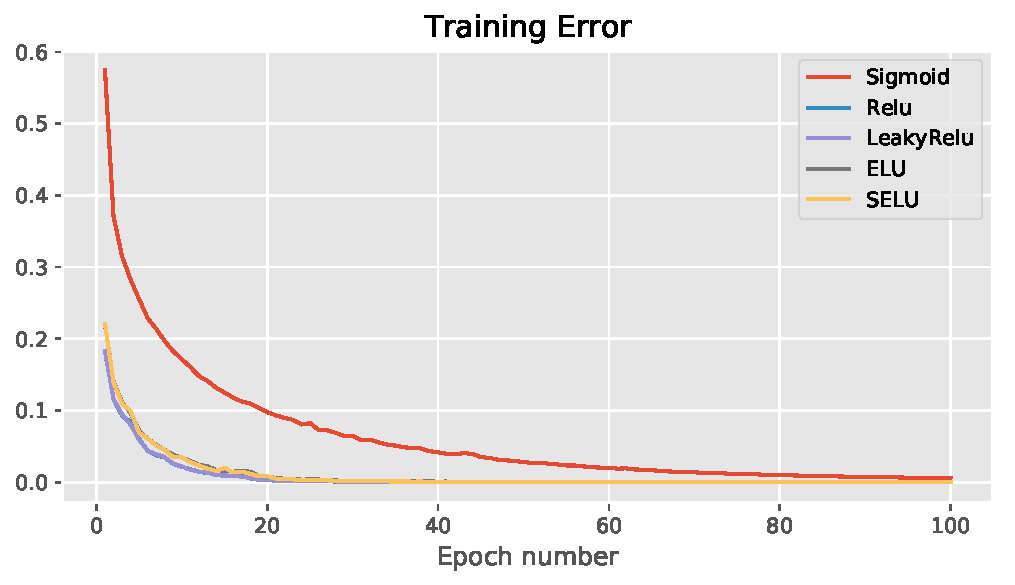
\includegraphics[width=\columnwidth]{activations_tr_error}}
\caption{Comparison of using different activation functions on training error}
\label{fig:act-tr-err}
\end{center}
\vskip -5mm
\end{figure} 

\begin{figure}[tb]
\vskip 5mm
\begin{center}
\centerline{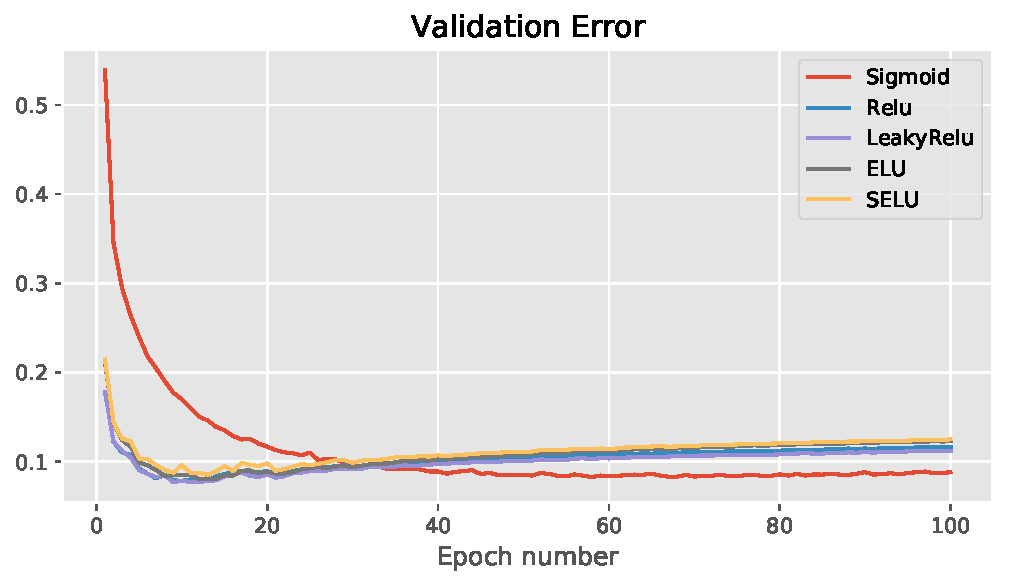
\includegraphics[width=\columnwidth]{activations_error}}
\caption{Comparison of using different activation functions on validation error}
\label{fig:act-val-err}
\end{center}
\vskip -5mm
\end{figure} 

\begin{figure}[tb]
\vskip 5mm
\begin{center}
\centerline{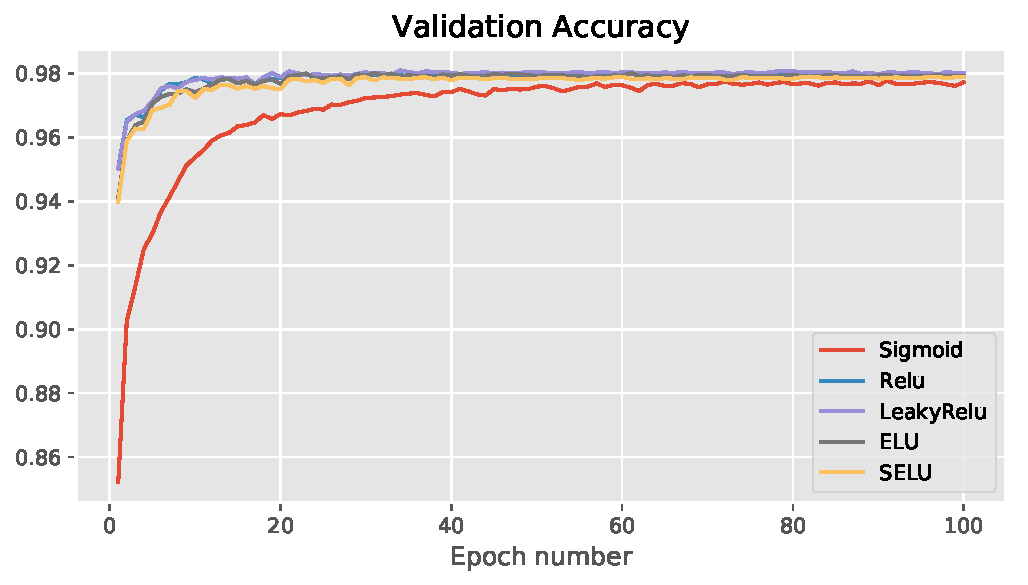
\includegraphics[width=\columnwidth]{activations_acc}}
\caption{Comparison of using different activation functions on validation accuracy}
\label{fig:act-val-acc}
\end{center}
\vskip -5mm
\end{figure} 

\begin{table}[tb]
\vskip 3mm
\begin{center}
\begin{small}
\begin{sc}
\begin{tabular}{lc}
\hline
\abovespace\belowspace
Activation function & Validation Accuracy  \\
\hline
\abovespace
Sigmoid    & 97.7  \\
ReLU & 98.0  \\
Leaky ReLU    & 98.0 \\
ELU    &  97.9\\
SELU   &  97.9 \\
\end{tabular}
\end{sc}
\end{small}
\caption{Validation accuracies using different activation functions}
\label{tab:act-table}
\end{center}
\vskip -3mm
\end{table}

\section{Deep neural network experiments}
\label{sec:dnnexpts}
\subsection{Changing network depth}
In the next part of our investigation, we look at the effects of network depth on validation accuracy. 

Using the results from the previous section, we decided to use Leaky ReLU as our hidden layer activation function. For $L \in \{2, 3, 4, 5, 6, 7, 8\}$, we trained a network with $L$ hidden layers using a batch size of 50 for 100 epochs, like before. Again, early-stopping was not implemented so we use the fully-trained network in our evaluations.

The graphs in this section (and the next subsection) are presented in the same order as in the previous section: training error (or learning curve), followed by validation error, and finally validation accuracy. Validation accuracy is summarised in table~\ref{tab:lay-table}.

We see from figure~\ref{fig:lay-tr-err} that changing network depth doesn't seem to impact how quickly the different networks learn; all networks seem to have fully fit to the training data by epoch 40. 

Figure~\ref{fig:lay-val-err} shows the two layer model having the lowest validation error, but this doesn't lead to good performance, as seen in table~\ref{tab:lay-table}. Again, we hypothesise that this model is making weaker predictions on the whole than the deeper networks. From this table, we see that the seven layer network has the highest validation accuracy. We suspect that the eight layer network overfits to the training data so much so as to cause the most probable class for certain examples to change. This would cause a lower validation accuracy than the seven layer model. 

\begin{figure}[tb]
\vskip 5mm
\begin{center}
\centerline{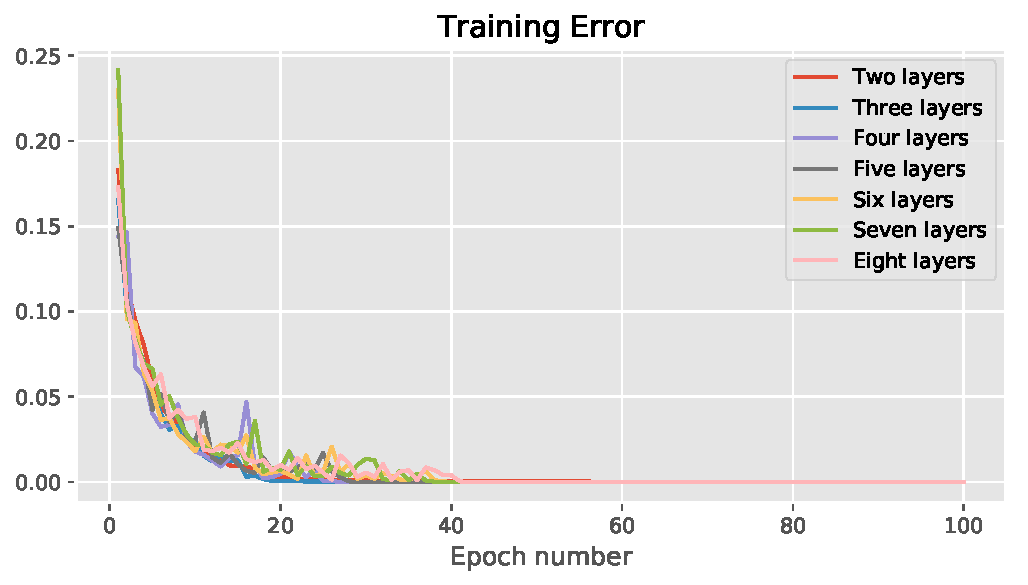
\includegraphics[width=\columnwidth]{layers_tr_error}}
\caption{Comparison of network depth on training error}
\label{fig:lay-tr-err}
\end{center}
\vskip -5mm
\end{figure} 

\begin{figure}[tb]
\vskip 5mm
\begin{center}
\centerline{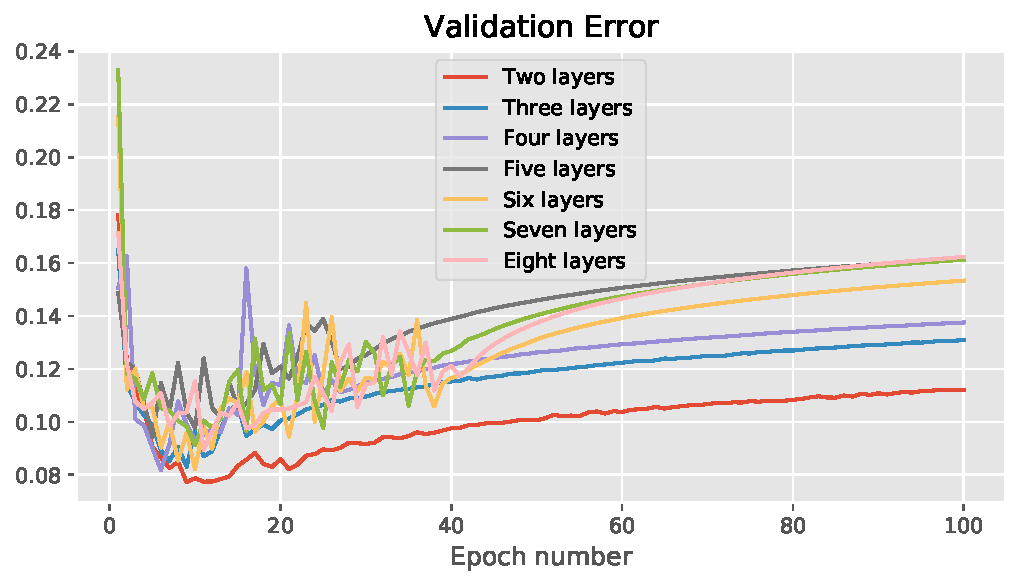
\includegraphics[width=\columnwidth]{layers_error}}
\caption{Comparison of network depth on validation error}
\label{fig:lay-val-err}
\end{center}
\vskip -5mm
\end{figure} 

\begin{figure}[tb]
\vskip 5mm
\begin{center}
\centerline{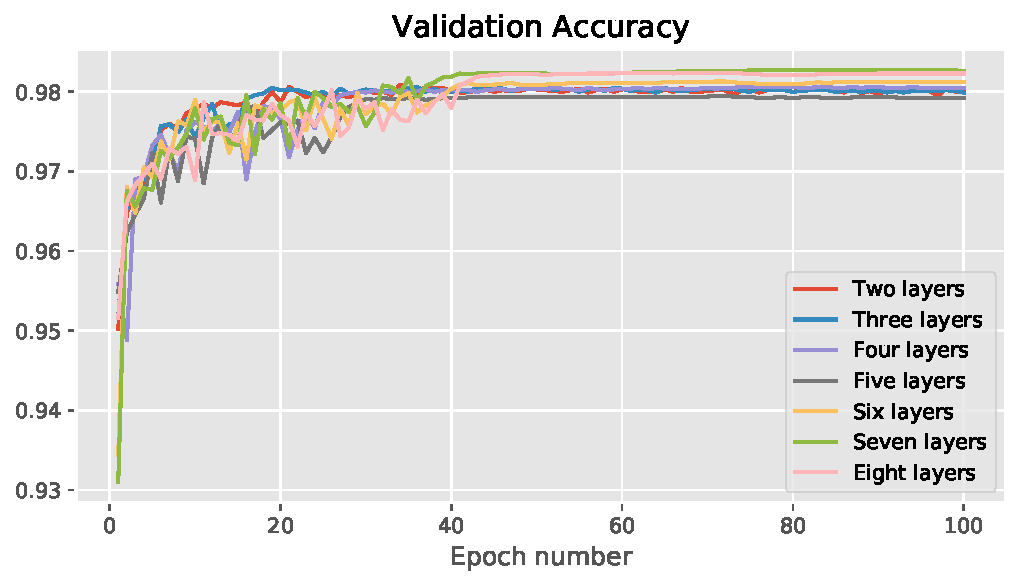
\includegraphics[width=\columnwidth]{layers_acc}}
\caption{Comparison of network depth on validation accuracy}
\label{fig:lay-val-acc}
\end{center}
\vskip -5mm
\end{figure}

\begin{table}[tb]
\vskip 3mm
\begin{center}
\begin{small}
\begin{sc}
\begin{tabular}{lc}
\hline
\abovespace\belowspace
Number of hidden layers & Validation Accuracy  \\
\hline
\abovespace
Two    & 98.0  \\
Three  & 98.0  \\
Four    & 98.0 \\
Five    &  97.9\\
Six   &  98.1 \\
Seven	  & 98.3 \\
Eight    & 98.2 \\
\end{tabular}
\end{sc}
\end{small}
\caption{Validation accuracies with different network depths}
\label{tab:lay-table}
\end{center}
\vskip -3mm
\end{table}
\subsection{Changing weights initialisation}
In this subsection, we explore the effects of changing the weights initialisation on validation accuracy. Again, using the results from the previous section, we decided to use a network with seven hidden layers, using the Leaky ReLU activation function for hidden layers. 

We explored three different weights initialisations: FanIn, FanOut and Glorot. FanIn sets uniformly-distributed weights so that the variance of the weights for a layer is independent of the number of incoming connections. FanOut sets uniformly-distributed weights so that the variance of the weights for a layer is independent of the number of outgoing connections. Glorot initialisation makes a compromise between the two.

Table~\ref{tab:init-table} shows the Glorot initialisation providing the best performance. We suspect this is because this initialisation keeps weights in a more suitable range so that the network has the chance to learn in more depth. 
\begin{figure}[tb]
\vskip 5mm
\begin{center}
\centerline{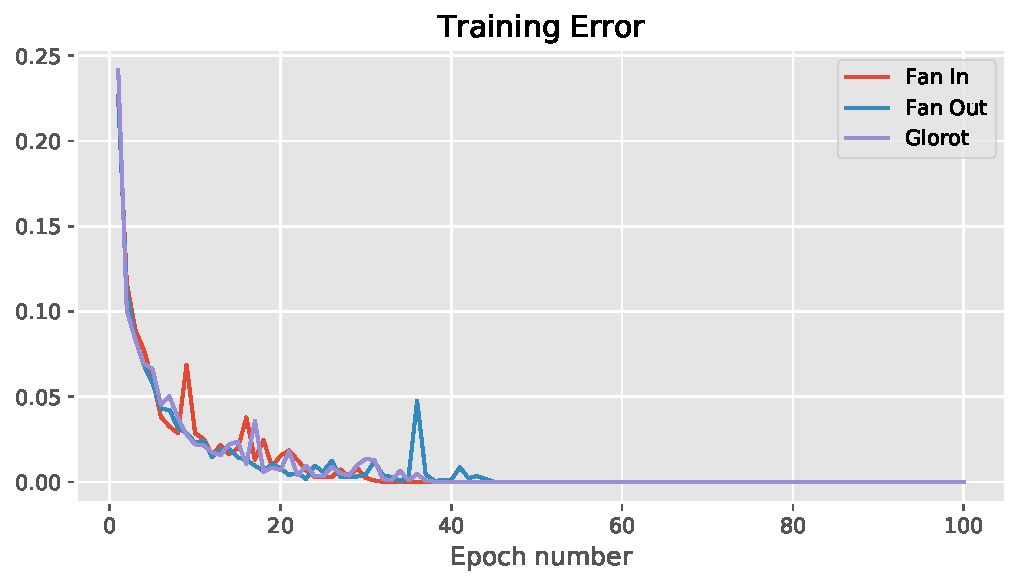
\includegraphics[width=\columnwidth]{init_tr_error}}
\caption{Comparison of different weights initialisations on training error}
\label{fig:init-tr-err}
\end{center}
\vskip -5mm
\end{figure} 

\begin{figure}[tb]
\vskip 5mm
\begin{center}
\centerline{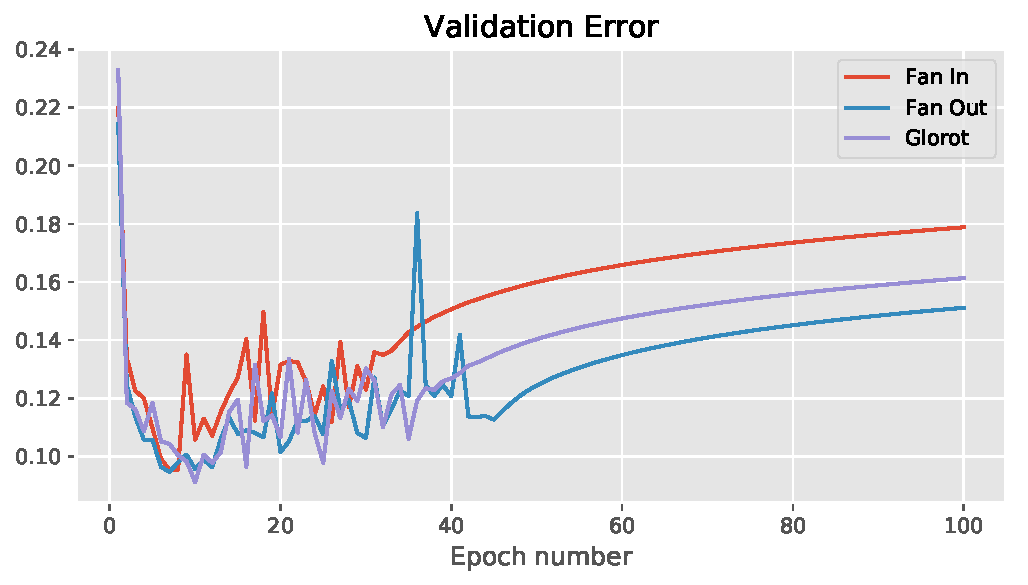
\includegraphics[width=\columnwidth]{init_error}}
\caption{Comparison of different weights initialisations on validation error}
\label{fig:init-val-err}
\end{center}
\vskip -5mm
\end{figure} 

\begin{figure}[tb]
\vskip 5mm
\begin{center}
\centerline{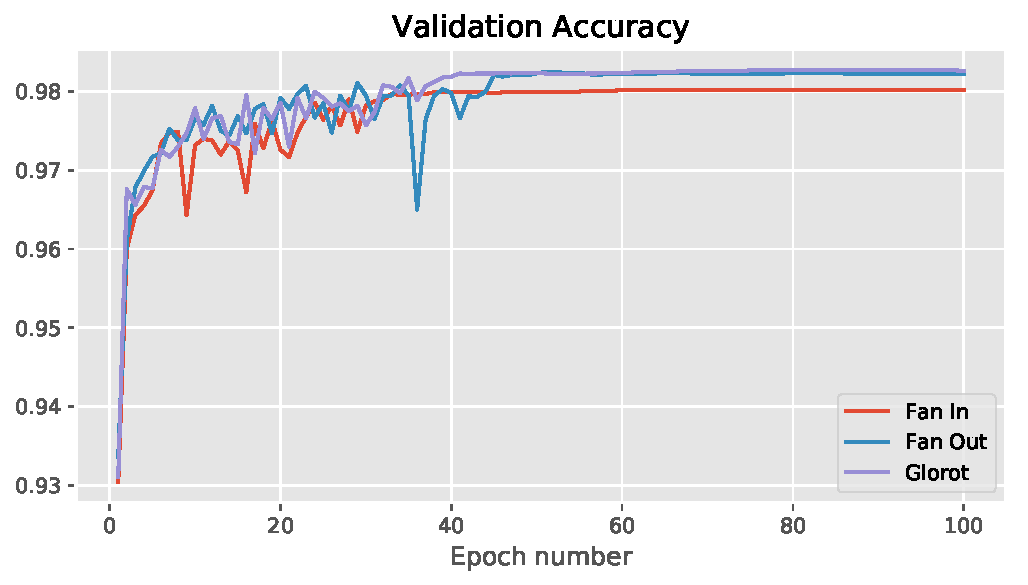
\includegraphics[width=\columnwidth]{init_acc}}
\caption{Comparison of different weights initialisations on validation accuracy}
\label{fig:init-val-acc}
\end{center}
\vskip -5mm
\end{figure} 

\begin{table}[tb]
\vskip 3mm
\begin{center}
\begin{small}
\begin{sc}
\begin{tabular}{lc}
\hline
\abovespace\belowspace
Weights initialisation & Validation Accuracy  \\
\hline
\abovespace
FanIn    & 98.0  \\
FanOut  & 98.2  \\
Glorot    & 98.3 \\
\end{tabular}
\end{sc}
\end{small}
\caption{Validation accuracies with different weights initialisations}
\label{tab:init-table}
\end{center}
\vskip -3mm
\end{table}

\section{Conclusions}
\label{sec:concl}
From our experiments, we conclude that in a network with two hidden layers, using the Leaky ReLU activation function provides the highest validation accuracy. This provided better results than the baseline (sigmoid) due to there no longer being a vanishing gradient.  Using this activation function, but varying depth (i.e. number of hidden layers) showed us that using seven hidden layers generalised the best. Changing the weights initialisation seemed to have a small impact on validation accuracy: with FanIn performing worse than FanOut and Glorot. 

Further work could look at whether similar results hold for different data sets (apart from network depth, which we hypothesise is largely dependent on the task at hand). Additionally, we could explore self-normalising networks \citep{Klambauer17} and investigate how network depth affects learning in this case. 
\bibliography{report-refs}

\end{document} 


% This document was modified from the file originally made available by
% Pat Langley and Andrea Danyluk for ICML-2K. This version was
% created by Lise Getoor and Tobias Scheffer, it was slightly modified  
% from the 2010 version by Thorsten Joachims & Johannes Fuernkranz, 
% slightly modified from the 2009 version by Kiri Wagstaff and 
% Sam Roweis's 2008 version, which is slightly modified from 
% Prasad Tadepalli's 2007 version which is a lightly 
% changed version of the previous year's version by Andrew Moore, 
% which was in turn edited from those of Kristian Kersting and 
% Codrina Lauth. Alex Smola contributed to the algorithmic style files.  
